\documentclass[border=4pt]{standalone}
\usepackage{amsmath,amssymb,tikz}
\usetikzlibrary{arrows.meta}
\definecolor{figB}{RGB}{31,90,166}\definecolor{figR}{RGB}{176,48,48}\definecolor{figG}{RGB}{46,125,50}\definecolor{figO}{RGB}{214,120,20}
\begin{document}
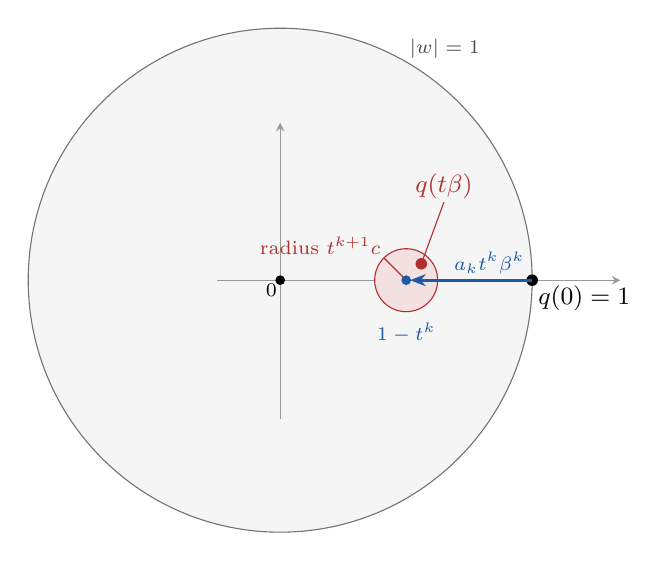
\begin{tikzpicture}[scale=1.6,>={Stealth[length=2mm]}]
% value plane of q; unit length = 2
\fill[black!4] (0,0) circle (2);
\draw[thin,black!40,-stealth] (-0.5,0)--(2.7,0);
\draw[thin,black!40,-stealth] (0,-1.1)--(0,1.25);
\draw[black!55] (0,0) circle (2); \node[font=\scriptsize,black!70,above right,inner sep=1pt] at (60:2) {$|w|=1$};
\fill (0,0) circle (1.1pt) node[below left,font=\scriptsize,inner sep=1pt]{$0$};
% leading-order motion 1 -> 1 - t^k
\fill (2,0) circle (1.3pt) node[below right,font=\small,inner sep=2pt]{$q(0)=1$};
% error disk
\fill[figR!15] (1,0) circle (0.25); \draw[figR] (1,0) circle (0.25);
\draw[figR,thin] (1,0)--++(135:0.25) node[pos=1,above left,font=\scriptsize,inner sep=1pt]{radius $t^{k+1}c$};
\draw[->,very thick,figB] (2,0)--(1.03,0);
\fill[figB] (1,0) circle (1.1pt);
\node[figB,font=\scriptsize,above,inner sep=2pt] at (1.66,0) {$a_kt^k\beta^k$};
\node[figB,font=\scriptsize,below] at (1,-0.26) {$1-t^k$};
\fill[figR] (1.12,0.13) circle (1.3pt);
\draw[figR,thin] (1.12,0.13)--(1.3,0.62) node[above,font=\small,inner sep=1pt]{$q(t\beta)$};
\end{tikzpicture}
\end{document}
